\documentclass{standalone}
\usepackage{tikz}
\usepackage{ctex,siunitx}
\setCJKmainfont{Noto Serif CJK SC}
\usepackage{tkz-euclide}
\usepackage{amsmath}
\usetikzlibrary{patterns, calc,3d}
\usetikzlibrary {decorations.pathmorphing,decorations.pathreplacing,decorations.shapes}
\tikzset{label style/.append style={font=\small}}
\begin{document}
\small
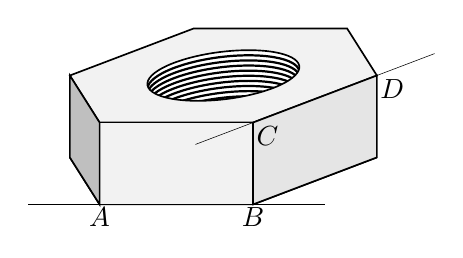
\begin{tikzpicture}[>=latex,scale=1.3,inner sep=1pt]
  \foreach \y in {0.45,0.4,0.35,0.3,0.25,0.2,0.15,0.1,0.05}
  {
    \begin{scope}[z={(45:5mm)},canvas is zx plane at y=\y]
      \draw[thick](0,0)circle(0.7);
    \end{scope}
  }
  \begin{scope}[z={(45:5mm)},canvas is zx plane at y=0.5]
    \draw[semithick,fill=lightgray!20,even odd rule]
      ( 30:1.5)--( 90:1.5)coordinate(A)--(150:1.5)coordinate(B)--(210:1.5)coordinate(C)--(270:1.5)coordinate(D)--(330:1.5)--cycle
      (0,0)circle(0.7);
    \draw[very thin](90:1.5)--++(30:0.7);
  \end{scope}
  \begin{scope}[z={(45:5mm)},canvas is zx plane at y=-0.3]
    \draw[semithick]
      ( 90:1.5)coordinate(A')--(150:1.5)coordinate(B')--(210:1.5)coordinate(C')--(270:1.5)coordinate(D');
    \draw[very thin]([yshift=7mm]B')--([yshift=-7mm]C');
  \end{scope}
  \draw[semithick,fill=lightgray!40](A)node[below right]{$D$}--(A')--(B')--(B)node[below right]{$C$}--cycle;
  \draw[semithick,fill=lightgray!20](B)--(B')node[below]{$B$}--(C')node[below]{$A$}--(C)--cycle;
  \draw[semithick,fill=lightgray](C)--(C')--(D')--(D)--cycle;
  \begin{scope}[z={(45:5mm)},canvas is zx plane at y=0.5]
    \draw[very thin](150:1.5)--++(30:-0.7);
  \end{scope}
\end{tikzpicture}
\end{document}